\documentclass[ignorenonframetext,]{beamer}
\setbeamertemplate{caption}[numbered]
\setbeamertemplate{caption label separator}{: }
\setbeamercolor{caption name}{fg=normal text.fg}
\beamertemplatenavigationsymbolsempty
\usepackage{lmodern}
\usepackage{amssymb,amsmath}
\usepackage{ifxetex,ifluatex}
\usepackage{fixltx2e} % provides \textsubscript
\ifnum 0\ifxetex 1\fi\ifluatex 1\fi=0 % if pdftex
  \usepackage[T1]{fontenc}
  \usepackage[utf8]{inputenc}
\else % if luatex or xelatex
  \ifxetex
    \usepackage{mathspec}
  \else
    \usepackage{fontspec}
  \fi
  \defaultfontfeatures{Ligatures=TeX,Scale=MatchLowercase}
\fi
% use upquote if available, for straight quotes in verbatim environments
\IfFileExists{upquote.sty}{\usepackage{upquote}}{}
% use microtype if available
\IfFileExists{microtype.sty}{%
\usepackage{microtype}
\UseMicrotypeSet[protrusion]{basicmath} % disable protrusion for tt fonts
}{}
\newif\ifbibliography
\hypersetup{
            pdftitle={Joining data frames in R using dplyr},
            pdfauthor={Erika Braithwaite, PhD},
            pdfborder={0 0 0},
            breaklinks=true}
\urlstyle{same}  % don't use monospace font for urls
\usepackage{color}
\usepackage{fancyvrb}
\newcommand{\VerbBar}{|}
\newcommand{\VERB}{\Verb[commandchars=\\\{\}]}
\DefineVerbatimEnvironment{Highlighting}{Verbatim}{commandchars=\\\{\}}
% Add ',fontsize=\small' for more characters per line
\usepackage{framed}
\definecolor{shadecolor}{RGB}{248,248,248}
\newenvironment{Shaded}{\begin{snugshade}}{\end{snugshade}}
\newcommand{\KeywordTok}[1]{\textcolor[rgb]{0.13,0.29,0.53}{\textbf{#1}}}
\newcommand{\DataTypeTok}[1]{\textcolor[rgb]{0.13,0.29,0.53}{#1}}
\newcommand{\DecValTok}[1]{\textcolor[rgb]{0.00,0.00,0.81}{#1}}
\newcommand{\BaseNTok}[1]{\textcolor[rgb]{0.00,0.00,0.81}{#1}}
\newcommand{\FloatTok}[1]{\textcolor[rgb]{0.00,0.00,0.81}{#1}}
\newcommand{\ConstantTok}[1]{\textcolor[rgb]{0.00,0.00,0.00}{#1}}
\newcommand{\CharTok}[1]{\textcolor[rgb]{0.31,0.60,0.02}{#1}}
\newcommand{\SpecialCharTok}[1]{\textcolor[rgb]{0.00,0.00,0.00}{#1}}
\newcommand{\StringTok}[1]{\textcolor[rgb]{0.31,0.60,0.02}{#1}}
\newcommand{\VerbatimStringTok}[1]{\textcolor[rgb]{0.31,0.60,0.02}{#1}}
\newcommand{\SpecialStringTok}[1]{\textcolor[rgb]{0.31,0.60,0.02}{#1}}
\newcommand{\ImportTok}[1]{#1}
\newcommand{\CommentTok}[1]{\textcolor[rgb]{0.56,0.35,0.01}{\textit{#1}}}
\newcommand{\DocumentationTok}[1]{\textcolor[rgb]{0.56,0.35,0.01}{\textbf{\textit{#1}}}}
\newcommand{\AnnotationTok}[1]{\textcolor[rgb]{0.56,0.35,0.01}{\textbf{\textit{#1}}}}
\newcommand{\CommentVarTok}[1]{\textcolor[rgb]{0.56,0.35,0.01}{\textbf{\textit{#1}}}}
\newcommand{\OtherTok}[1]{\textcolor[rgb]{0.56,0.35,0.01}{#1}}
\newcommand{\FunctionTok}[1]{\textcolor[rgb]{0.00,0.00,0.00}{#1}}
\newcommand{\VariableTok}[1]{\textcolor[rgb]{0.00,0.00,0.00}{#1}}
\newcommand{\ControlFlowTok}[1]{\textcolor[rgb]{0.13,0.29,0.53}{\textbf{#1}}}
\newcommand{\OperatorTok}[1]{\textcolor[rgb]{0.81,0.36,0.00}{\textbf{#1}}}
\newcommand{\BuiltInTok}[1]{#1}
\newcommand{\ExtensionTok}[1]{#1}
\newcommand{\PreprocessorTok}[1]{\textcolor[rgb]{0.56,0.35,0.01}{\textit{#1}}}
\newcommand{\AttributeTok}[1]{\textcolor[rgb]{0.77,0.63,0.00}{#1}}
\newcommand{\RegionMarkerTok}[1]{#1}
\newcommand{\InformationTok}[1]{\textcolor[rgb]{0.56,0.35,0.01}{\textbf{\textit{#1}}}}
\newcommand{\WarningTok}[1]{\textcolor[rgb]{0.56,0.35,0.01}{\textbf{\textit{#1}}}}
\newcommand{\AlertTok}[1]{\textcolor[rgb]{0.94,0.16,0.16}{#1}}
\newcommand{\ErrorTok}[1]{\textcolor[rgb]{0.64,0.00,0.00}{\textbf{#1}}}
\newcommand{\NormalTok}[1]{#1}
\usepackage{graphicx,grffile}
\makeatletter
\def\maxwidth{\ifdim\Gin@nat@width>\linewidth\linewidth\else\Gin@nat@width\fi}
\def\maxheight{\ifdim\Gin@nat@height>\textheight0.8\textheight\else\Gin@nat@height\fi}
\makeatother
% Scale images if necessary, so that they will not overflow the page
% margins by default, and it is still possible to overwrite the defaults
% using explicit options in \includegraphics[width, height, ...]{}
\setkeys{Gin}{width=\maxwidth,height=\maxheight,keepaspectratio}

% Prevent slide breaks in the middle of a paragraph:
\widowpenalties 1 10000
\raggedbottom

\AtBeginPart{
  \let\insertpartnumber\relax
  \let\partname\relax
  \frame{\partpage}
}
\AtBeginSection{
  \ifbibliography
  \else
    \let\insertsectionnumber\relax
    \let\sectionname\relax
    \frame{\sectionpage}
  \fi
}
\AtBeginSubsection{
  \let\insertsubsectionnumber\relax
  \let\subsectionname\relax
  \frame{\subsectionpage}
}

\setlength{\parindent}{0pt}
\setlength{\parskip}{6pt plus 2pt minus 1pt}
\setlength{\emergencystretch}{3em}  % prevent overfull lines
\providecommand{\tightlist}{%
  \setlength{\itemsep}{0pt}\setlength{\parskip}{0pt}}
\setcounter{secnumdepth}{0}

\title{Joining data frames in R using dplyr}
\subtitle{RLadies Montreal}
\author{Erika Braithwaite, PhD}
\date{March 15, 2018}

\begin{document}
\frame{\titlepage}

\begin{frame}[fragile]{What is joining?}

We often run into scenarios where we need to join two data frames
together. Let's say we had some students who were given an IQ test at a
career fair. Some of the students showed up at on both days, but not
all. They were given unique alphabetic identifiers (A-Q)

Set up

\begin{Shaded}
\begin{Highlighting}[]
\CommentTok{#install.packages('pacman')}
\NormalTok{pacman}\OperatorTok{::}\KeywordTok{p_load}\NormalTok{(knitr, kableExtra, formattable, data.table, dplyr, }
\NormalTok{               rmarkdown, magrittr, xtable)}
\end{Highlighting}
\end{Shaded}

Make some data

\begin{Shaded}
\begin{Highlighting}[]
\NormalTok{day1 =}\StringTok{  }\KeywordTok{data.table}\NormalTok{(}\DataTypeTok{ID=}\NormalTok{LETTERS[}\DecValTok{1}\OperatorTok{:}\DecValTok{12}\NormalTok{], }\DataTypeTok{IQ=}\KeywordTok{round}\NormalTok{(}\KeywordTok{rnorm}\NormalTok{(}\DecValTok{12}\NormalTok{, }\DecValTok{100}\NormalTok{, }\DecValTok{15}\NormalTok{),}\DecValTok{2}\NormalTok{))}

\NormalTok{day2 =}\StringTok{  }\KeywordTok{data.table}\NormalTok{(}\DataTypeTok{ID=}\NormalTok{LETTERS[}\DecValTok{6}\OperatorTok{:}\DecValTok{17}\NormalTok{],}\DataTypeTok{IQ=}\KeywordTok{round}\NormalTok{(}\KeywordTok{rnorm}\NormalTok{(}\DecValTok{12}\NormalTok{, }\DecValTok{100}\NormalTok{, }\DecValTok{20}\NormalTok{),}\DecValTok{2}\NormalTok{))}
\end{Highlighting}
\end{Shaded}

There are 12 individuals on day 1 and 12 individuals on day 2. 17 people
have a single measurement while 5 have 2 measurements

\end{frame}

\begin{frame}[fragile]{Our data}

ID

IQ

A

92.75

B

96.33

C

118.41

D

110.60

E

102.74

F

103.95

G

94.56

H

77.81

I

127.07

J

106.77

K

107.98

L

130.19

ID

IQ

F

122.96

G

140.90

H

100.29

I

128.33

J

103.18

K

93.63

L

128.85

M

85.09

N

126.77

O

143.69

P

158.16

Q

118.72

Let's explore the three(ish) types of joins in \texttt{dplyr}

\end{frame}

\begin{frame}[fragile]{Mutating joins}

\begin{block}{Add a new variables to one table from matching rows in
another}

\begin{itemize}
\tightlist
\item
  \texttt{left\_join}: Primary key is left data frame
\item
  \texttt{right\_join}: Primary key is right data frame
\item
  \texttt{inner\_join}: Retains rows in both data frame
\item
  \texttt{full\_join}: Retains all rows
\end{itemize}

Left, right and full joins are considered outer joins because when a row
doesn't match in an outer new, the new variables are filled with missing
values

\end{block}

\end{frame}

\begin{frame}[fragile]{Filtering joins}

\begin{block}{Filter observations from the primary based on whether they
are present in the secondary table}

\begin{itemize}
\tightlist
\item
  \texttt{semi\_join}: retains rows in the primary table that are also
  present in secondary table
\item
  \texttt{anti\_join}: retains rows in the primary that are not present
  in the secondary table
\end{itemize}

Filtering joins almost act like a filter in that the number of rows can
change, but not the columns

\end{block}

\end{frame}

\begin{frame}[fragile]{Set operations}

\begin{block}{Combines operations in the dataset as if they were set
elements. Much like filtering joins, they do not add new columns. Set
operations use combinations of observations from both data frames to
create a new data frame}

\begin{itemize}
\tightlist
\item
  \texttt{intersect}: retains rows ONLY if they appear in both data
  frames
\item
  \texttt{union}: retains rows that appear in EITHER data frames
\item
  \texttt{setdiff}: retains rows that ONLY appear in the primary data
  frame but not the second
\end{itemize}

\end{block}

\end{frame}

\begin{frame}[fragile]{Main arguments}

\begin{Shaded}
\begin{Highlighting}[]
\KeywordTok{right_join}\NormalTok{(x, y, }\DataTypeTok{by =} \OtherTok{NULL}\NormalTok{, }\DataTypeTok{copy =} \OtherTok{FALSE}\NormalTok{, }\DataTypeTok{suffix =} \KeywordTok{c}\NormalTok{(}\StringTok{'.x'}\NormalTok{, }\StringTok{'.y'}\NormalTok{), ...)}
\end{Highlighting}
\end{Shaded}

\begin{itemize}
\tightlist
\item
  \texttt{y} and \texttt{y} are the two data frames we are joining
\item
  \texttt{by} = primary key variable (typically a unique identifier)
  which can be one or several columns. The foreign key is the
  indentifier in the secondary table, which will be matched to the
  primary tables based on the primary key.
\item
  \texttt{copy} =
\item
  \texttt{suffix} will add a suffix to columns when they have the same
  name, e.g. \texttt{x.IQ} and \texttt{y.IQ}.
\end{itemize}

\end{frame}

\begin{frame}[fragile]{Mutating joins}

\begin{Shaded}
\begin{Highlighting}[]
\NormalTok{left =}\StringTok{ }\KeywordTok{left_join}\NormalTok{(day1, day2, }\DataTypeTok{by =} \StringTok{'ID'}\NormalTok{)}
\NormalTok{right =}\StringTok{ }\KeywordTok{right_join}\NormalTok{(day1, day2, }\DataTypeTok{by =} \StringTok{'ID'}\NormalTok{)}
\NormalTok{inner=}\StringTok{ }\KeywordTok{inner_join}\NormalTok{(day1, day2, }\DataTypeTok{by =} \StringTok{'ID'}\NormalTok{)}
\NormalTok{full =}\StringTok{ }\KeywordTok{full_join}\NormalTok{(day1, day2, }\DataTypeTok{by =} \StringTok{'ID'}\NormalTok{)}
\end{Highlighting}
\end{Shaded}

\begin{figure}
\centering
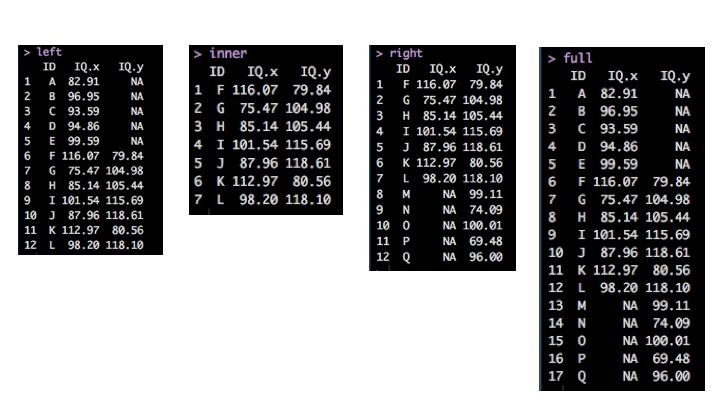
\includegraphics{graphs/mutate.png}
\caption{}
\end{figure}

\end{frame}

\begin{frame}[fragile]{Filtering joins}

\begin{Shaded}
\begin{Highlighting}[]
\NormalTok{semi =}\StringTok{ }\KeywordTok{semi_join}\NormalTok{(day1, day2, }\DataTypeTok{by =} \StringTok{'ID'}\NormalTok{)}
\NormalTok{anti =}\StringTok{ }\KeywordTok{anti_join}\NormalTok{(day1, day2, }\DataTypeTok{by =} \StringTok{'ID'}\NormalTok{)}
\end{Highlighting}
\end{Shaded}

\begin{figure}
\centering
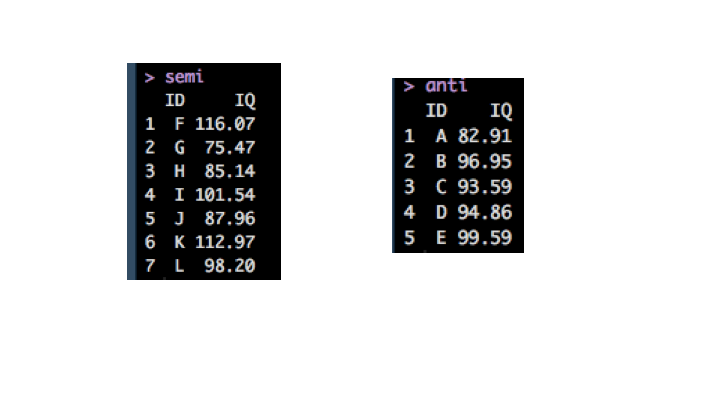
\includegraphics{graphs/filter.png}
\caption{}
\end{figure}

\end{frame}

\begin{frame}[fragile]{Set operations}

\begin{Shaded}
\begin{Highlighting}[]
\NormalTok{semi =}\StringTok{ }\KeywordTok{semi_join}\NormalTok{(day1, day2, }\DataTypeTok{by =} \StringTok{'ID'}\NormalTok{)}
\NormalTok{anti =}\StringTok{ }\KeywordTok{anti_join}\NormalTok{(day1, day2, }\DataTypeTok{by =} \StringTok{'ID'}\NormalTok{)}
\end{Highlighting}
\end{Shaded}

\begin{figure}
\centering
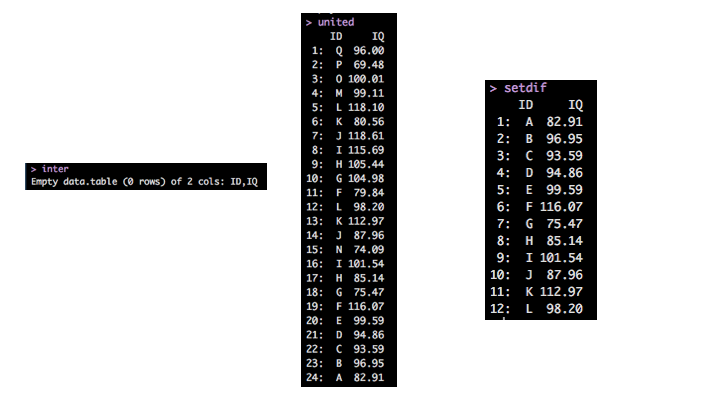
\includegraphics{graphs/set.png}
\caption{}
\end{figure}

\end{frame}

\begin{frame}[fragile]{dplyr versus \ldots{}}

\begin{block}{Base R: \texttt{rbind}, and \texttt{cbind}}

\begin{itemize}
\tightlist
\item
  Slower than \texttt{dplyr}
\item
  Can't handle lists of data frames
\item
  \texttt{rbind} returns an error when columns are not identical
\item
  \texttt{.id} arguments allows you to specify a name for each source
  data frame
\end{itemize}

\end{block}

\begin{block}{Data.table: \texttt{data.table::merge}}

While this point is contentious, if you've been a long standing
tidyversalist, then you might find \texttt{data.table::merge} syntax
more difficult to learn. Some people prefer \texttt{dplyr} because

\begin{itemize}
\tightlist
\item
  tells you what keys you're merging of (if not supplied)
\item
  rows are kept in existing order
\item
  also works with database tables
\end{itemize}

\end{block}

\end{frame}

\begin{frame}{When joining can get tricky\ldots{}}

\begin{itemize}
\tightlist
\item
  Joining columns having the same name but different encoding (UTF-8
  vs.~Latin)
\item
  Joining columns having different storage types (factors, integers,
  bit64, dates)
\end{itemize}

The consequences can vary, but dplyr might

\begin{itemize}
\tightlist
\item
  Set all the values to NA
\item
  Coerce a column to another type
\item
  Fail to recognize columns that match resulting in rows being dropped
\end{itemize}

\end{frame}

\begin{frame}[fragile]{More!}

There are additional types of joins not covered here: rolling joins,
scaling joins

Rolling joins are used in circumstances where you want to join
observations based on logical arguments (i.e.~range of date).

If you want to join 3 or more tables, go check out how a \texttt{list}
and \texttt{reduce} from \texttt{base\ R} or \texttt{purrr::reduce} can
help you.

\end{frame}

\end{document}
